Graph the initial temperature profile $u(x, 0)$. What does this mean in terms of the bar's initial temperature?

\begin{solution}\ \\\\
    If we let $L = \pi$, then our initial temperature profile is given below:

    \begin{figure}[h]
        \centering
        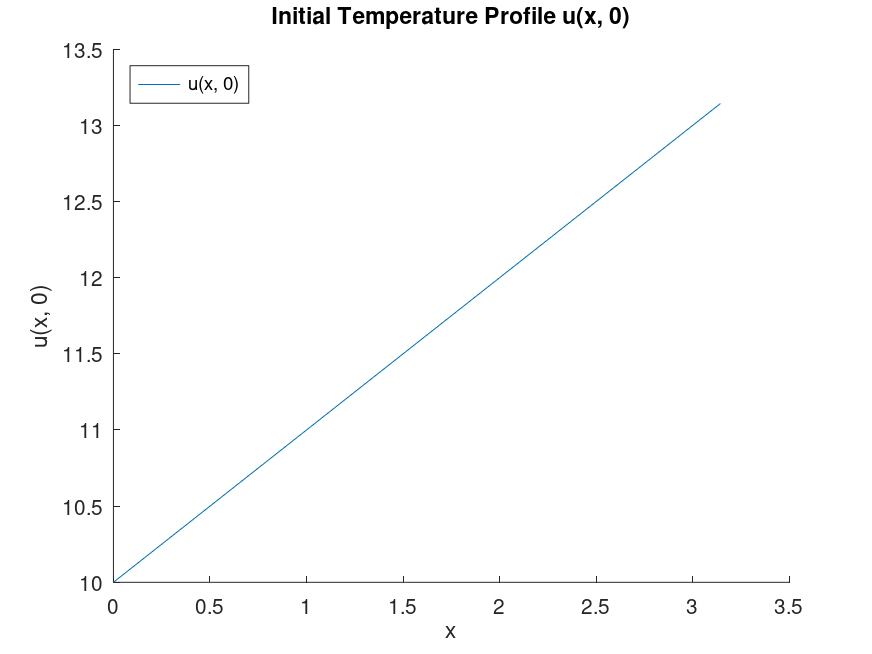
\includegraphics[width=0.7\textwidth]{problem1b_initial_temperature_profile.png}
        \caption{Initial temperature profile for $L = \pi$}
    \end{figure}
    \ \\

    In terms of the bar's initial temperature, we see that the bar temperature is lowest at $x = 0$ (the end presumably 
    submerged in a bath), increases linearly between $x = 0$ and $x = L$, and is highest (with a temperature of 
    $(10 + \pi)^{\circ}$) at the insulated end.
    \ \\
\end{solution}